\documentclass[a4paper,11pt]{article}

% Identificação
\newcommand{\pbtitulo}{Raspberry PI Pico com MicroPython}
\newcommand{\pbversao}{1.1}

\usepackage{../sty/tutorial}

%----------------------------------------------------------------------
% Início do Documento
%----------------------------------------------------------------------
\begin{document}

\maketitle % mostrar o título
\thispagestyle{fancy} % habilitar o cabeçalho/rodapé das páginas

%-----------------------------------------------------------------------------
% RESUMO DO ARTIGO
%-----------------------------------------------------------------------------

\begin{abstract}
\initial{R}\textbf{aspberry Pi Pico é uma placa com microcontrolador de baixo custo e alto desempenho que se destaca por seu tamanho reduzido e por oferecer uma alternativa acessível para projetos de hardware personalizados. É o primeiro microcontrolador desenvolvido pela Raspberry Pi Foundation e é baseado no chip RP2040, projetado pela própria fundação. A adoção do MicroPython no Raspberry Pi Pico apresenta várias vantagens, como a facilidade de programação e a rapidez no desenvolvimento de protótipos, devido à sintaxe concisa e legibilidade do Python.}
\end{abstract}

%-----------------------------------------------------------------------------
% CONTEÚDO DO ARTIGO
%-----------------------------------------------------------------------------
\section{Introdução}
Uma das principais vantagens de utilizar MicroPython para programar o Raspberry Pi Pico é a capacidade de executar comandos interativos em tempo real por meio do REPL (Read-Eval-Print Loop), sendo possível testar códigos e funções instantaneamente. Além disso, a linguagem Python possui uma vasta coleção de bibliotecas e módulos que podem ser facilmente integrados aos projetos, o que expande consideravelmente as possibilidades de uso do Pico em uma variedade de aplicações, incluindo automação residencial, robótica, sensores e muito mais.
\begin{figure}[H]
	\centering
	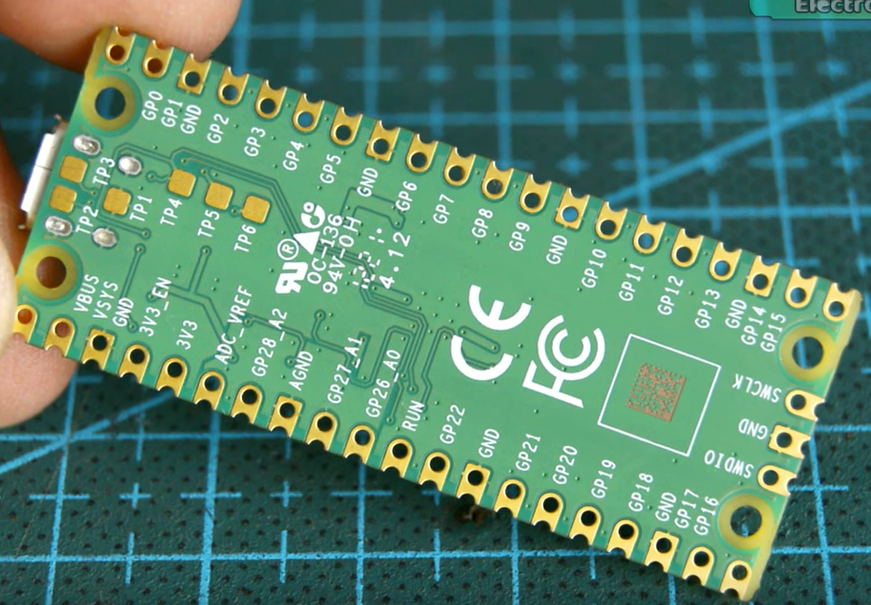
\includegraphics[width=0.5\textwidth]{imagem/PicoTraseira}
	\caption{Raspberry Pi Pico}
\end{figure}

Outro ponto significativo é a facilidade com que novos usuários e programadores podem começar a usar o MicroPython no Raspberry Pi Pico. A linguagem é conhecida por ser acessível a iniciantes, tornando a curva de aprendizado mais suave em comparação com outras linguagens mais complexas. Isso se traduz em uma rampa mais rápida para a criação de projetos eletrônicos e de programação, tornando o Pico uma opção atraente para educação, hobbistas e até mesmo para desenvolvedores de protótipos profissionais.

Em termos de recursos de hardware, o Raspberry Pi Pico oferece interfaces digitais flexíveis, permitindo a conexão com uma variedade de dispositivos e sensores externos. Sua arquitetura inclui uma configuração de memória generosa para um microcontrolador e vem com suporte tanto para MicroPython quanto para C/C++, garantindo versatilidade e desempenho adequados para uma gama de projetos de microcontroladores. Com essas características, o Raspberry Pi Pico com MicroPython representa uma combinação poderosa para a criação de projetos inovadores e complexos, mantendo um nível de simplicidade e acessibilidade para todos os níveis de habilidade.

\section{Projetos para a prática}
Aprender a programar com MicroPython por meio de exemplos práticos traz vantagens significativas, especialmente para aqueles que estão começando ou deseja ver resultados rápidos. Exemplificando, imagine que um estudante ou entusiasta queira automatizar uma estufa. Com MicroPython, seria possível programar o Raspberry Pi Pico para controlar a umidade e a temperatura, lendo dados de sensores em tempo real e ajustando um sistema de irrigação ou de controle de clima automaticamente. A implementação desse tipo de projeto ganha em simplicidade e clareza com a concisão da linguagem Python, e a imediata retroalimentação fornecida pelo REPL do MicroPython facilita a depuração e o aperfeiçoamento contínuo do código.

Outra vantagem prática de aprender MicroPython se revela na velocidade com que se pode passar da ideia ao protótipo funcional. Por exemplo, um projeto de robótica educacional onde os alunos estejam construindo um pequeno robô móvel. O uso do MicroPython permite aos alunos focar nos conceitos de lógica de programação e interação com componentes de hardware sem a sobrecarga de linguagens mais complexas ou de baixo nível. 

Isso significa que podemos dedicar mais tempo a entender como os motores funcionam e como controlá-los, ou como utilizar sensores para que o robô reaja ao ambiente. Assim, o MicroPython torna-se um facilitador de aprendizado e inovação, permitindo uma transição quase direta entre a teoria e a prática.

\textbf{ATENÇÃO}: Em todos os projetos descritos utilizaremos uma placa de prototipagem, \textit{jumpers} - fios para conexão (quantidade conforme vista no diagrama dos projetos) e um Raspberry PI Pico já configurado e iniciado para aceitar a programação MicroPython (veja diversos tutoriais e vídeos na Internet que ensinam como realizar este processo), que não serão descritos nos materiais necessários.

\subsection{Projeto 1 - Controlar um LED}

Este projeto possui os seguintes materiais: \vspace{-1em}
\begin{itemize}
	\item 1 LED vermelho
	\item 1 Resistor de 220 $\Omega$
\end{itemize}

\begin{figure}[H]
	\centering
	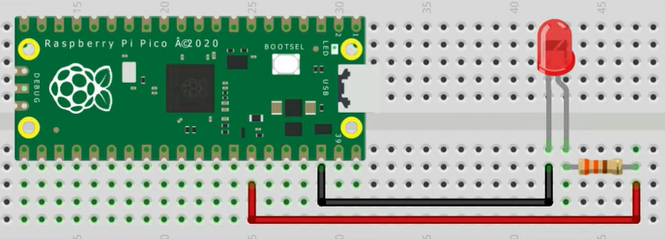
\includegraphics[width=0.6\textwidth]{imagem/PicoProj1}
	\caption{Esquemático para o Projeto 1}
\end{figure}

Ligações dos \textit{jumpers}: \vspace{-1em}
\begin{itemize}
	\item VERMELHO: para a placa na GP28
	\item PRETO: para a placa na GND
\end{itemize}

\begin{lstlisting}
from machine import Pin
import utime

led1 = Pin(28, Pin.OUT)
delay = .40
while True:
	led1.value(1)
	utime.sleep(delay)
	led1.value(0)
	utime.sleep(delay)
\end{lstlisting}

\subsection{Projeto 2 - Controlar vários LEDs}

Este projeto possui os seguintes materiais: \vspace{-1em}
\begin{itemize}
	\item 5 LEDs vermelho
	\item 5 Resistores de 220 $\Omega$
\end{itemize}

\begin{figure}[H]
	\centering
	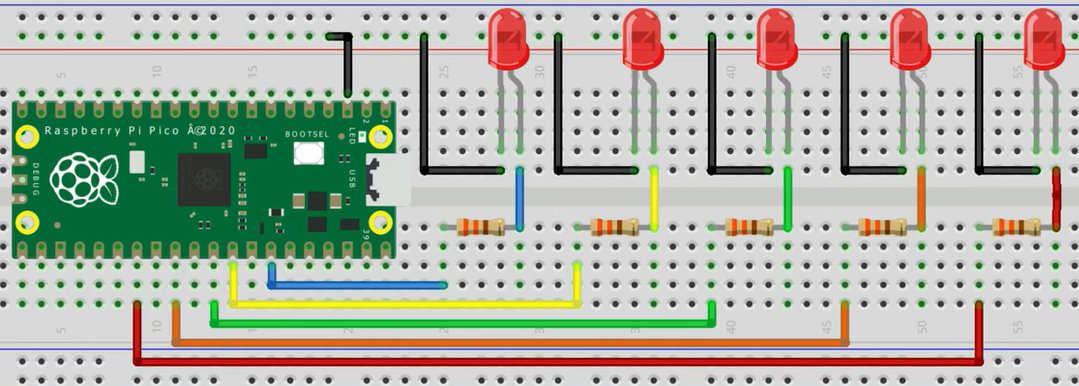
\includegraphics[width=0.8\textwidth]{imagem/PicoProj2}
	\caption{Esquemático para o Projeto 2}
\end{figure}

Ligações dos \textit{jumpers}: \vspace{-1em}
\begin{itemize}
	\item AZUL: para a placa na GP28
	\item AMARELO: para a placa na GP27
	\item VERDE: para a placa na GP26
	\item LARANJA: para a placa na GP22
	\item VERMELHO: para a placa na GP21
	\item PRETO: para a placa na GND
\end{itemize}

\begin{lstlisting}
from machine import Pin
import utime

led1 = Pin(28, Pin.OUT)
led2 = Pin(27, Pin.OUT)
led3 = Pin(26, Pin.OUT)
led4 = Pin(22, Pin.OUT)
led5 = Pin(21, Pin.OUT)
delay = .40

while True:
	led1.value(1)
	led2.value(0)
	led3.value(0)
	led4.value(0)
	led5.value(0)
	utime.sleep(delay)
	led1.value(0)
	led2.value(1)
	led3.value(0)
	led4.value(0)
	led5.value(0)
	utime.sleep(delay)
	led1.value(0)
	led2.value(0)
	led3.value(1)
	led4.value(0)
	led5.value(0)
	utime.sleep(delay)
	led1.value(0)
	led2.value(0)
	led3.value(0)
	led4.value(1)
	led5.value(0)
	utime.sleep(delay)
	led1.value(0)
	led2.value(0)
	led3.value(0)
	led4.value(0)
	led5.value(1)
	utime.sleep(delay)
\end{lstlisting}

\subsection{Projeto 3 - LED que acende e apaga}

Este projeto possui os seguintes materiais: \vspace{-1em}
\begin{itemize}
	\item 1 LED vermelho
	\item 1 PushButton
	\item 1 Resistor de 220 $\Omega$
\end{itemize}

\begin{figure}[H]
	\centering
	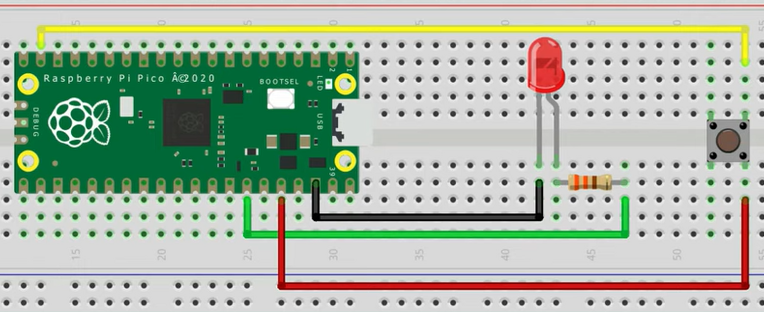
\includegraphics[width=0.6\textwidth]{imagem/PicoProj3}
	\caption{Esquemático para o Projeto 3}
\end{figure}

Ligações dos \textit{jumpers}: \vspace{-1em}
\begin{itemize}
	\item AMARELO: Lado A do Pushbutton para a placa na GP14
	\item VERMELHO: Lado B do Pushbutton para a placa em 3.3v
	\item VERDE: para a placa na GP28
	\item PRETO: para a placa na GND
\end{itemize}

\begin{lstlisting}
from machine import Pin
import time

led = Pin(28, Pin.OUT)
pbutton = Pin(14, Pin.IN, Pin.PULL_DOWN)

while True:
	if pbutton.value():
		led.toggle()
		time.sleep(0.5)
\end{lstlisting}

\subsection{Projeto 4 - Display OLED}

Este projeto possui os seguintes materiais: \vspace{-1em}
\begin{itemize}
	\item 1 Módulo display OLED LCD 0,96" (SSD1306)
\end{itemize}

\begin{figure}[H]
	\centering
	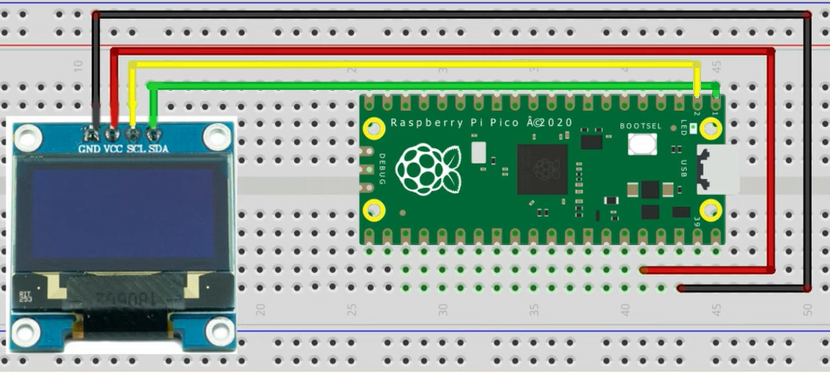
\includegraphics[width=0.6\textwidth]{imagem/PicoProj4}
	\caption{Esquemático para o Projeto 4}
\end{figure}

Ligações dos \textit{jumpers}: \vspace{-1em}
\begin{itemize}
	\item VERDE: SDA do OLED para a placa na GP0
	\item AMARELO: SCL do OLED para a placa na GP1
	\item VERMELHO: VCC do OLED para a placa em 3.3v
	\item PRETO: GND do OLED para a placa na GND
\end{itemize}

Nas opções do Thonny (Tools | Options... | Interpreter), verificar se está marcado "MicroPython (Raspberry Pi Pico)

Baixar as bibliotecas (Tools | Manage packages...):
\begin{itemize}
	\item micropython-ssd1306
	\item micropython-oled
\end{itemize}

\begin{lstlisting}
from machine import Pin, I2C
from ssd1306 import SSD1306_I2C
from oled import Write, GFX, SSD1306_I2C
from oled.fonts import ubuntu_mono_15, ubuntu_mono_20

WIDTH = 128
HEIGHT = 64

i2c = I2C(0, sda=Pin(0), scl=Pin(1), freq=400000)
oled = SSD1306_I2C(WIDTH, HEIGHT, i2c)

write15 = Write(oled, ubuntu_mono_15)
write20 = Write(oled, ubuntu_mono_20)

write20.text("OLED", 0, 0)
write15.text("Hello", 0, 20)
oled.text("Raspberry Pi Pico", 0, 40)
oled.show()
\end{lstlisting}

\subsection{Projeto 5 - Display OLED com Potenciômetro}

Este projeto possui os seguintes materiais: \vspace{-1em}
\begin{itemize}
	\item 1 Módulo display OLED LCD 0,96" (SSD1306)
	\item 1 Potenciômetro de 10 K$\Omega$
\end{itemize}

\begin{figure}[H]
	\centering
	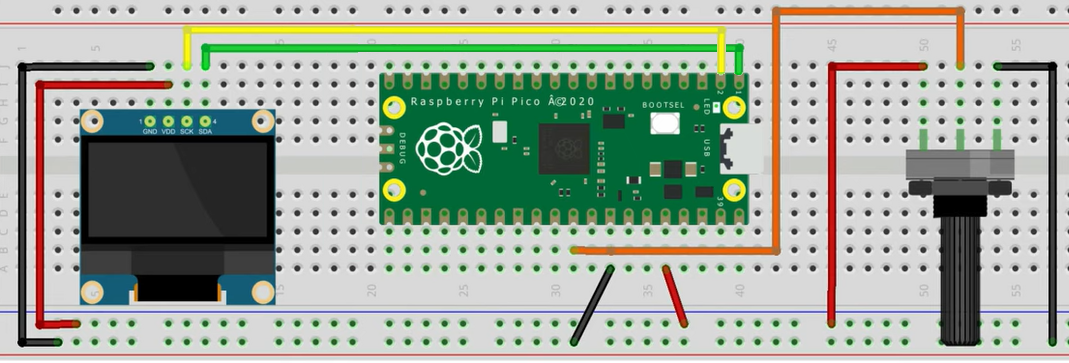
\includegraphics[width=0.6\textwidth]{imagem/PicoProj5}
	\caption{Esquemático para o Projeto 5}
\end{figure}

Ligações dos \textit{jumpers}: \vspace{-1em}
\begin{itemize}
	\item PRETO: primeira perna do potenciômetro para a placa na GND
	\item LARANJA: segunda perna do potenciômetro para a placa na GP26
	\item VERMELHO: terceira perna do potenciômetro para a placa em 3.3v
	\item VERDE: SDA do OLED para a placa na GP0
	\item AMARELO: SCL do OLED para a placa na GP1
	\item VERMELHO: VCC do OLED para a placa em 3.3v
	\item PRETO do GND do OLED para a placa na GND
\end{itemize}

\begin{lstlisting}
from machine import Pin, I2C
from ssd1306 import SSD1306_I2C
from oled import Write, GFX, SSD1306_I2C
from oled.fonts import ubuntu_mono_15, ubuntu_mono_20

WIDTH = 128
HEIGHT = 64

i2c = I2C(0, sda=Pin(0), scl=Pin(1), freq=400000)
oled = SSD1306_I2C(WIDTH, HEIGHT, i2c)

pot_val = machine.ADC(26)
fator_conversao = 3.3 / 65535

write15 = Write(oled, ubuntu_mono_15)
write20 = Write(oled, ubuntu_mono_20)

while True:
	dado = pot_val.read_u16() * fator_conversao
	oled.fill(0)
	write20.text("Valor: ", 0, 0)
	write15.text(str(round(dado,1)), 0, 20)
	oled.show()
\end{lstlisting}

\subsection{Projeto 6 - Sensor de Distância}

Este projeto possui os seguintes materiais: \vspace{-1em}
\begin{itemize}
	\item 1 Módulo display OLED LCD 0,96" (SSD1306)
	\item 1 Módulo Sensor Ultrassônico (HC-SR04)
\end{itemize}

\begin{figure}[H]
	\centering
	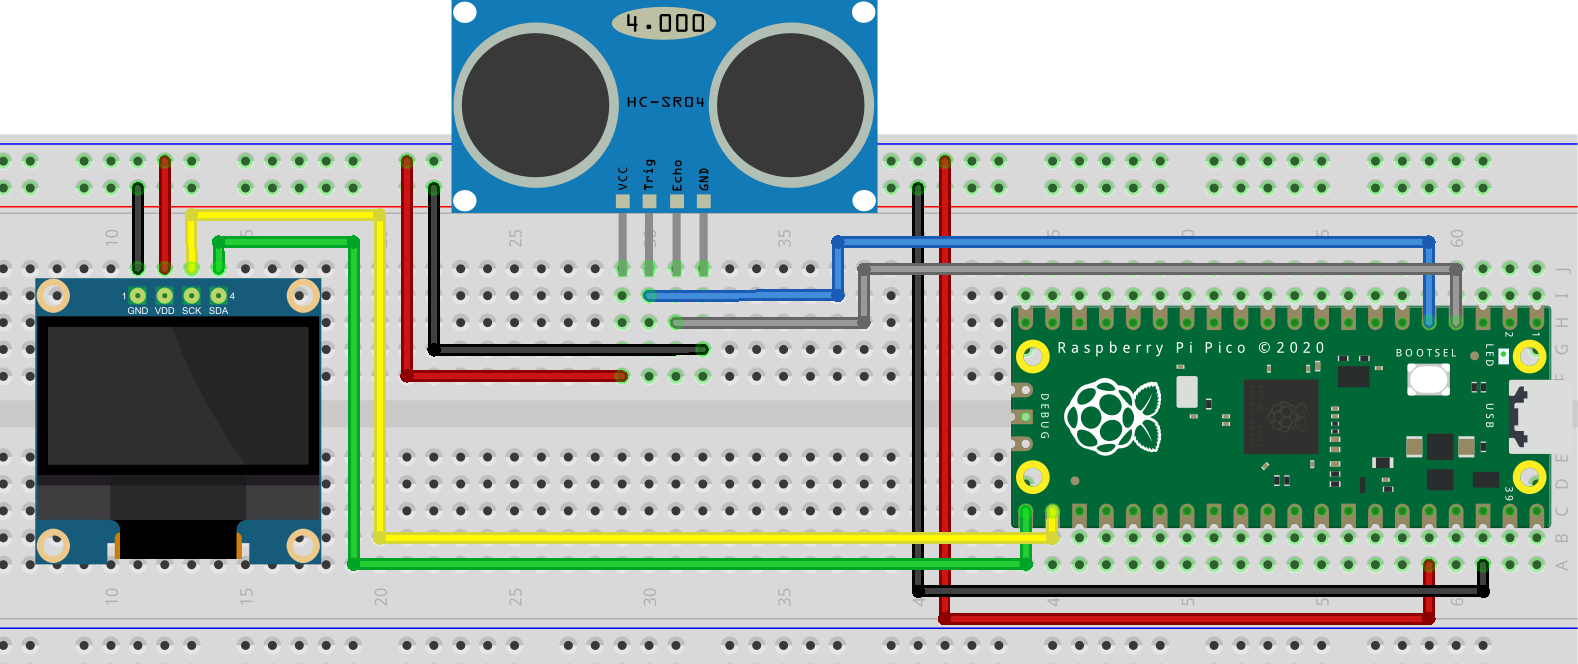
\includegraphics[width=0.7\textwidth]{imagem/PicoProj6}
	\caption{Esquemático para o Projeto 6}
\end{figure}

Ligações dos \textit{jumpers}: \vspace{-1em}
\begin{itemize}
	\item AZUL: Trigger do HC para a placa na GP13
	\item CINZA: ECHO do HC para a placa na GP2
	\item VERDE: SDA do OLED para a placa na GP0
	\item AMARELO: SCL do OLED para a placa na GP1
	\item VERMELHO: VCC do HC e OLED para a placa em 3.3v
	\item PRETO: GND do HC e OLED para a placa na GND
\end{itemize}

\begin{lstlisting}
from machine import Pin, I2C
from ssd1306 import SSD1306_I2C
from oled import Write, GFX, SSD1306_I2C
from oled.fonts import ubuntu_mono_15, ubuntu_mono_20
import utime

trigger = Pin(3, Pin.OUT)
echo = Pin(2, Pin.IN)

def distancia():
	tempo = 0
	trigger.low()
	utime.sleep_us(2)
	trigger.high()
	utime.sleep_us(5)
	trigger.low()
	while echo.value() == 0:
		signaloff = utime.tick_us()
	while echo.value() == 1:
		signalon = utime.tick_us()
	tempo = signalon - signaloff
	return tempo

WIDTH = 128
HEIGHT = 64

i2c = I2C(0, sda=Pin(0), scl=Pin(1), freq=400000)
oled = SSD1306_I2C(WIDTH, HEIGHT, i2c)

write15 = Write(oled, ubuntu_mono_15)
write20 = Write(oled, ubuntu_mono_20)

while True:
	distancia_cm = (distancia() * 0.0343) / 2
	oled.fill(0)
	write20.text("Distância: ", 0, 0)
	write15.text(str(round(distancia_cm,1)) + " cm", 0, 20)
	oled.show()
\end{lstlisting}

\subsection{Projeto 7 - Acender Lâmpada com LDR}

Este projeto possui os seguintes materiais: \vspace{-1em}
\begin{itemize}
	\item 1 Módulo LDR
	\item 1 Módulo Relay
	\item 1 Lâmpada, Bocal e Tomada (110/220v)
\end{itemize}

\begin{figure}[H]
	\centering
	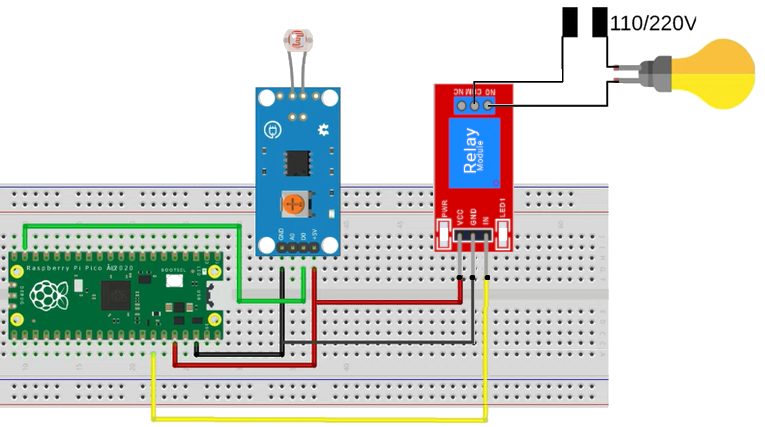
\includegraphics[width=0.8\textwidth]{imagem/PicoProj7}
	\caption{Esquemático para o Projeto 7}
\end{figure}

Ligações dos \textit{jumpers}: \vspace{-1em}
\begin{itemize}
	\item AMARELO: IN do Relay para a placa na GP28
	\item VERDE: D0 do LDR para a placa na GP14
	\item VERMELHO: da placa em 3.3v
	\item PRETO: para a placa na GND
	\item Ligação 1 do RELAY em 110/220v: NC para a Lâmpada
	\item Ligação 2 do RELAY em 110/220v: COM para a Tomada
\end{itemize}

\begin{lstlisting}
from machine import Pin
import time

relay = Pin(28, Pin.OUT)
ldr = Pin(14, Pin.IN, Pin.PULL_DOWN)

while True:
	if ldr.value():
		relay.value(1)
	else:
		relay.value(0)
	time.sleep(0.5)
\end{lstlisting}

\subsection{Projeto 8 - Alarme com Sensor de Proximidade}

Este projeto possui os seguintes materiais: \vspace{-1em}
\begin{itemize}
	\item 1 Módulo Sensor de Movimento - PIR (HC-SR501)
	\item 1 Sensor Buzzer (Passivo)
\end{itemize}

\begin{figure}[H]
	\centering
	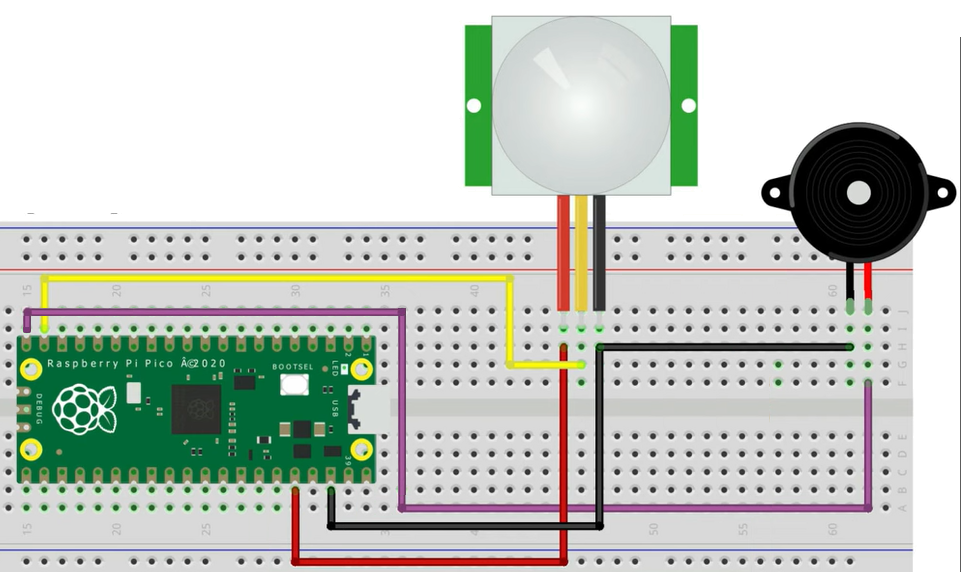
\includegraphics[width=0.6\textwidth]{imagem/PicoProj8}
	\caption{Esquemático para o Projeto 8}
\end{figure}

Ligações dos \textit{jumpers}: \vspace{-1em}
\begin{itemize}
	\item AMARELO: PIR para a placa na GP14
	\item ROXO: Buzzer para a placa na GP15
	\item VERMELHO: da placa em 3.3v
	\item PRETO: para a placa na GND
\end{itemize}

\begin{lstlisting}
from machine import Pin
import time

pir = Pin(14, Pin.IN, Pin.PULL_DOWN)
buzzer = Pin(15, Pin.OUT, Pin.PULL_DOWN)

while True:
    if pir.value():
        print("Movimento detectado")
        buzzer.value(1)
    else:
        print("Nenhum movimento detectado")

    time.sleep(1)
    buzzer.value(0)
\end{lstlisting}


\section{Conclusão}
O Raspberry Pi Pico é uma placa de microcontrolador notável por suas características robustas e custo acessível, rodando a linguagem de programação Python em sua variante MicroPython. Essa combinação oferece uma plataforma ideal para aprendizes, entusiastas e profissionais desenvolverem rapidamente protótipos funcionais. 

Com a facilidade de interação em tempo real através do REPL, programadores podem testar e ajustar seu código instantaneamente, promovendo um ciclo de aprendizagem e desenvolvimento mais ágil. O amplo suporte de bibliotecas Python disponíveis acelera a integração com uma variedade de sensores e atuadores, expandindo o leque de possíveis aplicações práticas em áreas como automação residencial, robótica e controle ambiental.

A simplicidade e acessibilidade da linguagem Python, junto com as funcionalidades oferecidas pelo MicroPython, tornam o Raspberry Pi Pico uma ferramenta de ensino e desenvolvimento excepcional. Projetos como a automação de uma estufa ou a criação de um robô educativo se tornam muito mais tangíveis, permitem que mesmo programadores iniciantes possam se concentrar nos aspectos lógicos e criativos da interação com o hardware, sem as complicações de linguagens mais complexas. 

Esta abordagem prática e orientada por exemplos facilita o aprendizado e a inovação, permite a transição rápida da teoria para a construção de projetos eletrônicos reais e complexos, satisfaz tanto a curiosidade quanto a necessidade de soluções práticas.

Sou um entusiasta do mundo \textbf{Open Source} e novas tecnologias. Qual a diferença entre Livre e Open Source? \underline{Livre} significa que esta apostila é gratuita e pode ser compartilhada a vontade. \underline{Open Source} além de livre todos os arquivos que permitem a geração desta (chamados de arquivos fontes) devem ser disponibilizados para que qualquer pessoa possa modificar ao seu prazer, gerar novas, complementar ou fazer o que quiser. Os fontes da apostila (que foi produzida com o LaTex) está disponibilizado no GitHub \cite{github}. Veja ainda outros artigos que publico sobre tecnologia através do meu Blog Oficial \cite{fernandoanselmo}.

%-----------------------------------------------------------------------------
% REFERÊNCIAS
%-----------------------------------------------------------------------------
\begin{thebibliography}{7}
  \bibitem{rur} 
  A peça conta a história de um brilhante cientista, chamado Rossum, que desenvolve uma substância química similar ao protoplasma. Utiliza essa substância para construção de humanoides (robôs), com o intuito de que estes sejam obedientes e realizem todo o trabalho físico.

  \bibitem{cs106a} 
  Curso de Metodologia da programação de Stanford \\
  \url{https://see.stanford.edu/Course/CS106A}
  
  \bibitem{openkareloficial} 
  Página do OpenKarel no GitHub \\
  \url{https://github.com/fernandoans/OpenKarel}
  
  \bibitem{bluej} 
  Editor BlueJ para Java \\
  \url{http://bluej.org/}

  	\bibitem{fernandoanselmo} 
	Fernando Anselmo - Blog Oficial de Tecnologia \\
	\url{http://www.fernandoanselmo.blogspot.com.br/}
	
	\bibitem{publicacao} 
	Encontre essa e outras publicações em \\
	\url{https://cetrex.academia.edu/FernandoAnselmo}
	
	\bibitem{github} 
	Repositório para os fontes da apostila \\
	\url{https://github.com/fernandoans/publicacoes}
\end{thebibliography}
  
\end{document}
